\section{Mathematische Grundbegriffe}



\subsection{Aussagen}

\subsubsection{Aussage}

Bevor wir über Aussagen reden, lohnt es sich kurz über das Definieren und Bezeichnen zu reden. Das Definieren ist das Befüllen eines Wortes oder Ausdrucks mit einer eindeutigen Bedeutung. Das Bezeichnen ist was ähhliches: das ist das Befüllen eines symbolischen Ausdrucks mit einer Bedeutung. 
 Eine Definition oder Bezeichnnung hat einen Gültigkeitsbereich. Man kann zum Beispiel schreiben: in meiner Abschlussarbeit nenne ich eine ganze Zahl schön, wenn sie durch $5$ teilbar ist. ``Schön'' wird somit zu  einer Abkürzung für ``ganze Zahl, die durch $5$ teilbar ist''. Wenn man bei der Diskussion eines Themas solche Art Zahlen öfter benötigt, kann man durch die Verwendung des Begriffs ``schön'' Aussagen kürzer fassen. Ein weiterer Vorteil ist, dass man interessante bzw. relevante Eigenschaften durch das Einführen der einschlägigen Definitionen konzeptualisiert und somit verdeutlicht und greifbar macht. Manche mathematische Strukturen werden mit Hilfe von gewissen Grundeigenschaften defininiert. Dann nennt man oft die Grundeigenschaften Axiome. Bei uns im Kurs werden Gruppen, Ringe, Körper und Vektorräume auf diese Weise eingeführt. Mathematische Fakten werden mit der Verwendung von Definitionen und Bezeichnungen als mathematische Aussagen formuliert. Das Bedeutet: rigorose Mathematik ist nichts anderes als eine Ansammlung von Definitionen, Bezeichnungen, Aussagen und deren Begrüdungen (die man, Beweise nennt). 

Nun zu Aussagen. Eine (mathematische) Aussage ist eine Behauptung (meistens in der Form eines Satzes, in dem man sowohl Worte als auch mathematische Formeln nutzen darf), die  entweder wahr oder falsch ist. Die Information darüber, ob die Aussage wahr oder falsch ist, nennt man den Wahrheitswert der Aussage. 
Hier Beispiele von Aussagen und Nicht-Aussagen: 
\begin{itemize}
	\item $ 2 < 1 $ (falsche Aussage)
	\item $ 2 = 1 $ (falsche Aussage)
	\item $ 2 > 1 $ (wahre Aussage)
	\item $11$ ist eine Primzahl (es ist eine Aussage, sobald festgelegt ist, was es heißt, Primzahl zu sein). 
	\item $0$ ist eine natürliche Zahl (Sobald man die Bedeutung des Begriffs natürliche Zahl geklärt hat, ist das eine Aussage. Ob wahr oder falsch, hängt davon ab, wie wir die natürlichen Zahlen definieren. Wenn man eine Theorie entwickelt oder eine Schrift verasst, entscheidet man selbst, mit welcher Bedeutung man Begriffe festlegt. Natürlich gibt es gewisse Standards wie man welche Fachbegriffe mit einer Bedeutung befüllt, aber auch die Freiheiten eigene Fachbegriffe im Kontext eigener Arbeit einzuführen)
	\item ``Hallo!'' (keine Aussage, weil hier nichts Behauptet wird)
	\item ``Was gibt's Neues?'' (keine Behauptung sondern eine Frage)
	\item ``$1$ und $2$ sind nah beieinander'' (ist zwar eine Behauptung, aber keine Aussage, denn was heißt schon nah beieinander zu sein? Wenn wir aber vorher definieren, dass zwei natürlich Zahlen nah beinander sind, wenn der Betrag ihrer Differenz höchstens eins ist, so wird zu einer wahren Aussage.)
	\item $(a+b)^2 = a^2 + 2 a b + b^2$ (hier fehlt die Erklärung, was eigentlich unter $a$ und $b$ gemeint ist. Wir könnten aber schreiben $(a+b)^2 = a^2 + 2 a b + b^2$ gilt für alle reellen Zahlen $a$ und $b$. Dann ist das eine wahre Aussage).
	\item $a^2 + b^2 =c^2$.  Ist keine Aussage, weil hier nicht geklärt worden ist, was $a, b $ und $c$ überhaupt ist. 
	item $E= m c^2$. Ebenso keine Aussage aus dem selben Grund. 
	\item ``Die Erde ist rund''. (schon eine sinnvolle Behauptung, aber keine mathematische, denn  weißt heißt eigentlich ganz genau ``Die Erde'' und was heißt ganz genau ``rund sein''?) 
\end{itemize}

Für Mathematik (mathematische Schriften) ist charakteristisch, dass man in den mathematischen Aussagen im Gegensatz zu anderen Wissenschaften überhaupt keinen Interpretationsspielraum zulässt. Denn Begriffe werden eindeutig geklärt. Sobald dass geschehen ist, sind auch die Wahrheitswerte der Aussage eindeutig. Je genauer bei einem Forschungsthema Begriffe festgelegt werden, desto mathematischer wird das Thema in der Regel. 


\begin{bem}[Betiteln mathematischer Aussagen] Beim Betiteln von bewiesenen mathematischen Aussagen gibt es die folgenden Tendenzen (die sich aus Tradition oder subjektiven Einschätzungen ergeben):
	\begin{itemize}
		\item Proposition: relativ einfach zu beweisen 
		\item Theorem, Satz: bemerkenswert oder schwer zu beweisen
		\item Lemma, Hilfssatz:  Hilfsaussage, die  technisch  ist und beim Beweis eines Theorems eingesetzt wird. 
	\end{itemize}
\end{bem}


\subsubsection{Logische Verknüpfungen}

Seien $ A $ und $ B $ Aussagen. Dann definiert man anhand von $ A $ und $ B $ die folgenden Aussagen:
\begin{itemize}
	\item $ A \wedge B $ Konjunktion (\glqq und\grqq) ist genau dann wahr, wenn sowohl $A$ als auch $B$ wahr ist. 
	\item $ A \vee B $ Disjunktion (\glqq oder\grqq) ist genau falsch, wenn sowohl $A$ als auch $B$ falsch ist. 
	\item $ A \Rightarrow B $ Implikation ist genau dann falsch, wenn $A$ wahr und $B$ falsch ist. 
	\item $ A \Leftrightarrow B $ Äquivalenz ist genau dann wahr, wenn die Wahrheitswerte von $A$ und $B$ gleich sind. 
	\item $ A \:\dot{\vee}\: B $ ausschließende Disjunktion ist gen dann wahr, wenn die Wahrheitswerte von $A$ und $B$ verschieden sind. 
	\item $ \neg A $, $ \bar{A} $ Negation (Verneinung) ist genau dann wahr, wenn $A$ falsch ist. 
\end{itemize}

\begin{bsp}\
	\begin{itemize}
		\item Für alle $ x,y \in \R$ gilt: $x = y \Rightarrow x^2 = y^2 $ (wahr)
		\item Für alle $ x,y \in \R$ gilt:  $x^2 = y^2 \Rightarrow x = y $ (falsch)	
	\end{itemize}
\end{bsp}

\clearpage
\subsection{Mengen}

\subsubsection{Menge}

Menge ist der Grundbegriff der Mathematik schlechthin. Im Prinzip kann man alle mathematischen Konzepte (Zahlen, Tupel usw.) auf dem Begriff der Menge aufbauend einführen. Das machen wir aber in diesem Kurs nicht, weil wir den übermäßigen und unnötigen Formalismus vermeiden wollen Die intuitive Beschreibung der Menge ist wie folgt: Eine Menge ist eine Ansammlung von unterscheidbaren Objekten; diese Objekte nennt man Elemente der Menge. Eine Menge $M$ ist genau dann eindeutig beschrieben, wenn man für jedes Objekt $x$ eindeutig beantworten kann, ob $x$ Element der Menge ist oder nicht. Die Menge $M=\{1,2,3\}$ etwa besteht aus genau drei Objekten - den natürlichen Zahlen $1$, $2$ und $3$. In diesem Fall ist ein Objekt $x$ genau dann Element der Menge $M$ wenn $x=1$ oder $x=2$ oder $x=3$ ist. Man kann auch Mengen einführen, deren Elemente ebenfalls Mengen sind, wie z.B. $\{\{1,2,3\},\{1,2\},\{2,3\}\}$. Die Angabe einer Menge beinhaltet keine Reihung deren Elemente. Das heißt: $\{1,2,3\}$ ist z.B. die selbe Menge wie $\{3,1,2\}$. Die Objekte, die durch die Beschreibung einer Menge in die Menge aufgenommen werden, haben auch keine Vielfachheit innerhalb der Menge. Das heißt z.B., dass $\{1,1,2,3\}$ die selbe Menge als $\{1,2,3\}$ ist. 

Wir werden im Folgenden nur mit der oben eingeführten intuitiven Beschreibung des Begriffs Menge arbeiten. Es gibt auch eine exakte Beschreibung mit Hilfe von Axiomen (definierenden Grundeigenschaften), die wir aber in diesem Kurs nicht diskutieren werden. 

Eine gängige Weise, Mengen zu definieren, ist durch die Auflistung ihrer Elemente. Dabei stehen die geschweiften Klammer für Mengen, die drei Punkte bedeuten \glqq usw\grqq.
\begin{itemize}
	\item $ \{1,2,5,7\} $
	\item $ \{1\} $
	\item $ \{1,\{2,5\},\{6\}\} $
	\item $ \{1,2,3,\ldots\} $
\end{itemize}
Ist $ x $ Element der Menge $ X $, so schreibt man $ x \in X $. Ist $ x $ kein Element der Menge $X$, so schreibt man $ x \notin X $. Die Lesart zu $x \in X$ ist: $x$ ist Element der Menge $X$. Die Lesart zu $x \not\in X$ ist: $x$ ist kein Element der Menge $X$. Hier und im Folgenden werden wir parallel zur Einführung neuer Begriffe oft auch Bezeichnungen für diese Begriffe einführen. Dadurch wird es möglich sein, über mathematische Themen mit der Verwendung der natürlichen Sprache (der Fachsprache der Mathematik) aber auch mit Hilfe von Formeln zu kommunizieren. 

Seien $ A $ und $ B $ Mengen. Dann ist $ A $ genau dann eine Teilmenge von $ B $, wenn jedes Element von $ A $ auch Element von $ B $ ist. Als Bezeichnung:  $ A \subseteq B :\Leftrightarrow \forall\: x \in A : x \in B $.\footnote{In einigen mathematischen Quellen bezeichnet man die Inklusion als $ \subset $ und nicht als $ \subseteq $. Es gibt aber auch Quellen, in denen $ \subset $ die strikte Inklusion bezeichnet. Daher ziehe ich persönlich $ \subseteq $ vor.}\footnote{Durch den Doppelpunkt in $:\Leftrightarrow$ wird verdeutlicht, dass wir hiermit eine neue Bezeichnung $\subseteq$ einführen. Das Gleiche macht man auch mit dem Gleichheitszeichen, indem man $:=$ schreibt.}  Zwei Mengen $ A $ und $ B $ heißen genau dann gleich, wenn $ A \subseteq B $ und $ B \subseteq A $ gilt. $ A $ heißt genau dann echte Teilmenge einer Menge $ B $, wenn $ A \subseteq B $ und $ A \neq B $ erfüllt sind. Bezeichnung: $ A \varsubsetneq B $.


Beispiel: $\{Mo, Di, Mi, Do, Fr, Sa, So \} $  ist die Menge der Wochentage und $\{Sa,So\}$ ist die Menge der Wochenendtage. Die Menge der Wochenendtage ist eine Teilmenge der Menge der Wochenendtage. 

\subsubsection{Zahlenmengen}

\begin{itemize}
	\item Wir nennen die Menge $\N := \{ 1,2,3,\ldots \} $ die Menge der natürlichen Zahlen. Die Definition des Begriffs natürliche Zahl sowie die Bedeutung der jeweiligen Bezeichnung $\N$ für die Menge der natürlichen Zahlen sind abhängig von einer konkreten Quelle. Manche Quellen definieren die Menge der natürlichen Zahlen als $ \set{0,1,2,\ldots} $, es ist mittlerweile sogar die ISO-Norm 80000-2, es gibt aber trotz der ISO-Norm sehr viele Quellen, in denen $0$ nicht in die Menge der natürlichen Zahl aufgenommen wird. Tendenziell wählt man  $\N = \{1,2,3,\ldots \}$ in der Analysis und $\N = \{0,1,2,\ldots\}$ in der theoretischen Informatik, Mengenlehre sowie der diskreten Mathematik.
	\item $ \N_0 := \{ 0,1,2,\ldots \} $
	\item Wir nennen $ \Z  := \{ 0,1,-1,2,-2,\ldots \} $ die Menge ganzer Zahlen. 
	\item Wir nennen die Menge $ \Q  := \{ \frac{p}{q} : p \in \Z, q \in \N \}$ die Menge rationaler Zahlen
	\item Die Definition der Menge $ \R $ reeller Zahlen wird in der Analysis gegeben. 
	\item Die Definition der Menge $\C$ der komplexen Zahlen wird in der Analysis gegeben. 
\end{itemize}

\noindent Für die oben eingeführten Menge gelten die Inklusionen $ \N \subseteq \N_0 \subseteq \Z \subseteq \Q \subseteq \R \subseteq \C $

\begin{bem}[Intervalle]
	Seien $ a,b \in \R $ mit $ a < b $. Dann werden dei verschiedenen Arten von  Intervallen wie folgt definiert:
	\begin{align*}
		[a,b] &:= \{ x \in \R : a \leq x \leq b \} & & \text{(abgeschlossenes Intervall mit den Endpunkten $a$ und $b$)}\\ 
		(a,b) &:= \{ x \in \R : a < x < b \}  &  &\text{(offenes Intervall mit den Endpunkten $a$ und $b$)}\\
		(a,b] &:= \{ x \in \R : a < x \leq b \} & & \text{(links offenes, rechts abgeschlossenes Intervall...)} \\ 
		[a,b) &:= \{ x \in \R : a \leq x < b \} & & \text{(links abgeschlossenes, recht offenens Intervall...)} 
	\end{align*}
	Es werden auch die folgenden unbeschränkten Intervalle eingeführt:
	\begin{align*}
	 [a,\infty) & := \{ x \in \R \,:\, x \ge a\},
	 \\  (a,\infty) &:= \{ x \in \R \,:\, x > a\},
	 \\ (-\infty,b] &:= \{ x\in \R\,:\, x \le b\},
	\\  (-\infty,b) &:= \{ x \in \R\,:\, x < b\}. 
	\end{align*} 
\end{bem}


\subsubsection{Definition durch eine Bedingung}

Eine weitere Weise, Mengen zu definieren, ist durch Bedingungen. Format:
\[
			 \{ \text{AUSDRUCK} \,  : \, \text{BEDINGUNG} \}
\]
Die Lesart für den Doppelpunkt ist ``sodass''  bzw.  ``mit der Bedingung''.  (In manchen Quellen wird ein Vertikalstrich an der Stelle des Doppelpunkts benutzt.)

Zum Beispiel beschreibt die Formel
 \[
 	\{ k^2 : k \in \N, \ k \, \text{ungerade} \} 
 \] die Menge aller Quadrate von positiven ungeraden ganzen Zahlen. Eine andere Beschreibung für dieselbe Menge ist 
 \[
 	\{  (2i -1)^2  \, :\, i \in \N\}.
 \] 



\subsubsection{Die leere Menge}

Die leere Menge ist die Menge, die keine Elemente enthält. Sie wird als $ \emptyset $ bezeichnet. 

\subsubsection{Potenzmenge}

Sei $ X $ eine Menge. Dann ist die Potenzmenge von $ X $ als die Menge aller Teilmengen von $ X $ definiert. Die Potenzmenge von $X$ bezeichnen wir als  $ 2^X $. Formal: $ 2^X := \{ A : A \subseteq X \} $. Die Wahl dieser Bezeichnung ist duch die Tatsache motiviert, dass im Fall einer $n$-elementigen Menge $X$ mit $n \in \N_0$, die Potenzmenge von $X$ genau $2^n$ Elemente hat. 


\subsubsection{Mengenoperationen}

Seien $ A,B $ Mengen. Dann heißt
\begin{itemize}
\item $ A \cap B := \{ x : (x \in A) \wedge (x \in B) \} $ Durchschnitt von $ A $ und $ B $
\item $ A \cup B := \{ x : (x \in A) \vee (x \in B) \} $ Vereinigung von $ A $ und $ B $
\item $ A \setminus B := \{ x : (x \in A) \wedge (x \notin B) \} $ Mengendifferenz von $ A $ und $ B $
\end{itemize}

\subsubsection{Disjunkte Mengen}

Seinen $ A,B $ Mengen. $ A $ und $ B $ heißen genau dann disjunkt, wenn $ A \cap B = \emptyset $.

\subsection{Tupel}

Für Objekte $ a,b $ kann man das \emph{geordnete Paar} $ (a,b) $ definieren. Für Objekte $ a,b,c,d $ definiert man die Gleichheit $ (a,b) = (c,d) $ durch $ a=c $ und $ b=d $. $ a $ heißt das erste Element des Paares $ (a,b) $ und $ b $ heißt das zweite Element.

Für Mengen $ X,Y $ definiert man das \emph{Kreuzprodukt} $ A \times B $ durch $ A \times B := \{ (x,y) : x \in X, y \in Y \} $. Analog definiert man geordnete Tripel und das Kreuzprodukt $ A \times B \times C $ von Mengen $ X,Y $ und $ Z $. Noch allgemeiner kann man für jedes $ n \in \N $ geordnete $ n $-Tupel $ (x_1,\ldots,x_n) $ einführen und das Kreuzprodukt $ X_1 \times \ldots \times X_n := \{ (x_1,\ldots,x_n) : x_1 \in X_1, \ldots , x_n \in X_n \} $ von Mengen $ X1,\ldots,X_n $.

Für eine Menge $ X $ führt man die Bezeichnung
\begin{equation*}
	X^n := \underbrace{X \times \ldots \times X}_{n \:\text{mal}} = \{ (x_1,\ldots,x_n) : x_1,\ldots,x_n \in X \}.
\end{equation*}
Das Element $ x_i $ mit $ i \in \is{1}{n} $ im $ n $-Tupel $ (x_1,\ldots,x_n) $ heißt die $ i $-te \emph{Komponente} des Tupels.

\begin{bsp} Geometrische Veranschaulichung einiger Tupel:
	\begin{itemize}
		\item $ [0,1] \times [0,2] $ ist Rechteck in $ \R^2 $\\
		$ \{ 0 \} \times [0,2] $ ist eine Kante dieses Rechtecks\\
		$ \{ 0,1 \} \times \{ 0,2 \} $ sind Eckpunkte dieses Rechtecks
		\item $ [0,1]^3 $ ist Würfel in $ \R^3 $\\
		$ [0,1]^2 \times \{ 0 \} $ ist eine Seitenfläche des Würfels\\
		$ [0,1]^2 \times \{ 1 \} $ ist gegenüberliegende Seitenfläche (Facette)\\
		$ \{ 0 \}^2 \times [0,1] $ ist eine Kante des Würfels
		\item $ [0,1]^4 $ ist ein 4-dimensionaler Würfel in $ \R^4 $
	\end{itemize}
\end{bsp}


\subsection{Abbildungen}

\subsubsection{Abbildung}

Seien $ X,Y $ Mengen. Eine Abbildung $ f $ von $ X $ nach $ Y $ ist eine Vorschrift, die jedem $ x \in X $ genau ein Element aus $ Y $ zuordnet. Dieses Element aus $ Y $ wird durch $ f(x) $ bezeichnet.
% 16.10.2014
Wenn $ f $ eine Abbildung von $ X $ nach $ Y $ ist, dann bezeichnet man das durch: $ f : X \to Y $. Die Menge $ X $ heißt der Definitionsbereich von $ f $, $ Y $ heißt der Wertebereich von $ f $.

%Beispiel:
%\begin{enumeration}
%\item Kekse
%\item Nüsse
%\item Riegel
%\end{enumeration}
%
%\begin{table}[h]
%	\begin{tabular}{c|c|c}
%		$ X $ & $ Y $ & $ Y $ \\
%		\hline
%		1 & Kekse & Kekse \\
%		2 & Kekse & Nüsse \\
%		3 & Kekse & Riegel
%	\end{tabular}
%\end{table}

\begin{itemize}
	\item $ f : \R \to \R$ mit $ f(x) := x^2 -2x + 7 $
	\item $ f : \R \setminus \{ 1 \} \to \R$ mit $f(x) := \frac{1}{x-1}$
	\item $ \sign: \R \to \R $ mit 
	\[
	 \sign(x) := \begin{cases} 1,  & \text{für} \ x>0, \\
	 0,  &\text{für} \ x=0, 
 \\ -1, & \text{für} \ x<0. \end{cases} 
	\]
	\item $ f : 2^{\N} \to \N$ mit $ f(A) := \min(A)$. Man hat für diese Abbildung  z.B. $ f( \{ 1,7,43 \} ) = 1 $
	\item $ f : \N \to 2^\N$ mit  $f(k) := \is{1}{k}$
\end{itemize}

Zwei Abbildungen $ f,g : X \to Y $ heißen gleich, falls $ f(x) = g(x) $ für alle $ x \in X $ gilt. Als $ Y^X $ bezeichnen wir die Menge aller Abbildungen von $ X $ nach $ Y $.

\subsubsection{Bild und Urbild}

Seien $ X,Y,A,B $ Mengen mit $ A \subseteq X $ und $ B \subseteq Y $. Sei $ f : X \to Y $. Dann heißt $ f(A) := \{ f(x) : x \in A \} $ das Bild von $ A $ bzgl. $ f $ und $ f^{-1}(B) := \{ x \in X : f(x) \in B \} $ das Urbild von $ B $ bzgl. $ f $.

\begin{bsp}
	Für die Abbildung $ f : \R \to \R $ mit $ f(x) := x^2 $ hat man 
	\[
		 f( [1,2] ) = \{ x^2 \,:\, 1 \le x \le 2\} = [1,4] .
	\]
\begin{center}
	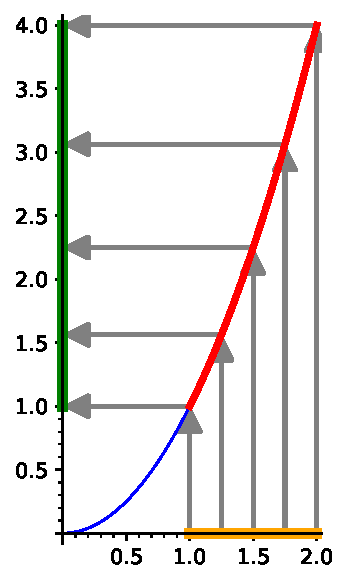
\includegraphics[width=0.3\textwidth]{sage/bild_abb.pdf}
\end{center} 
	
	Außerdem hat man die folgenen Urbilder: 
	
	\[
		 f^{-1}( [1,4] ) = \{ x \in \R \,:\, x^2  \in [1,4] \} = [1,2] \cup [-2,-1] .
	\] 
\begin{center}
	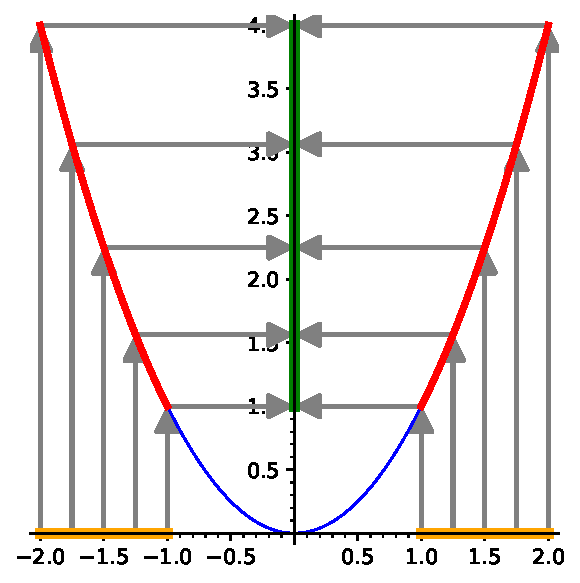
\includegraphics[width=0.6\textwidth]{sage/urbild_abb.pdf}
\end{center} 

und

		$ \begin{aligned}[t]
			f^{-1}( [-1,4] ) &= \{ x \in \R : f(x) \in [-1,4] \} \\
			&= \{ x \in \R : -1 \leq f(x) \leq 4 \} \\
			&= \{ x \in \R : -1 \leq x^2 \leq 4 \} \\
			&= \{ x \in \R : x^2 \leq 4 \} \\
			&= \{ x \in \R : |x| \leq 2 \} \\
			&= [-2,2]
		\end{aligned} $
\end{bsp}


\subsubsection{Injektivität, Surjektivität und Bijektivität}

Seien $ X,Y $ Mengen und sei $ f : X \to Y $. Dann heißt $ f $:
\begin{itemize}
	\item injektiv, falls für alle $ x_1, x_2 \in X : x_1 \neq x_2 $ die Bedingung $ f(x_1) \neq f(x_2) $ gilt.
	\item surjektiv, falls für jedes $ y \in Y $ ein $ x \in X $ mit der Eigenschaft $ f(x) = y $ existiert.
	\item bijektiv, falls $ f $ injektiv und surjektiv ist.
\end{itemize}

\begin{bsp}
	Untersuche folgende Funktionen auf Bijektivität:
	\begin{itemize}
		\item $ f : \R \to \R, f(x) := x^2 $ für alle $ x \in \R $\\
		surjektiv ? nein, $ -1 \neq f(x) $ für alle $ x \in \R $\\
		injektiv ? nein, $ f(x) = f(-x) $ für alle $ x \in \R $
		\item $ f : \R \to [0,+\infty), f(x) := x^2 $ für alle $ x \in \R $\\
		surjektiv ? ja\\
		injektiv ? nein (analog)
		\item $ f : \R \setminus \{ 0 \} \to \R, f(x) = \frac{1}{x} $ für alle $ x \in \R $\\
		surjektiv ? nein, 0 wird nicht angenommen\\
		injektiv ? ja
		\item $ f : \R \to \R, f(x) = 2x + 3 $ für alle $ x \in \R $\\
		bijektiv ? ja
	\end{itemize}
\end{bsp}

\subsubsection{Umkehrfunktion}

Seien $ X,Y $ Mengen und sei $ f : X \to Y $ bijektiv. Die Abbildung, die jedem $ y \in Y $ das eindeutige $ x \in X $ mit $ f(x) = y $ zuordnet, heißt die Umkehrabbildung von $ f $ und wird durch $ f^{-1} $ bezeichnet.

\begin{bsp}
	Die Umkehrung von $ f : \R \to \R : f(x) := 2x + 3 $ ist $ f^{-1}(x) = \frac{x-3}{2} $ $ ( x \in \R ) $.
\end{bsp}

\subsubsection{Komposition}

Seien $ X,Y,Z $ Mengen, $ f : X \to Y $ und $ g : Y \to Z $. Dann heißt $ g \circ f : X \to Z $ mit $ ( g \circ f )(x) := g( f(x) ) $ für alle $ x \in X $ die Komposition von $ g $ und $ f $.

\begin{bsp}
	Seien $ f : \R \to \R : f(x) = 2x + 3 $ für alle $ x \in \R $ und $ g : \R \to \R : g(x) = x^2 $ für alle $ x \in \R $. Dann ist $ ( f \circ g )(x) = 2x^2 + 3 $ und $ ( g \circ f )(x) = (2x + 3)^2 $.
\end{bsp}

\subsubsection{Identische Abbildung}

Sei $ X $ eine Menge. Dann heißt die Abbildung $ \id_X : X \to X $ mit $ \id_X(x) := x $ für alle $ x \in X $ die identische Abbildung auf $ X $. Man schreibt auch häufig $ \id $, wenn $ X $ nicht angegeben werden muss.

\begin{bem}
	Seien $ X,Y $ Mengen und sei $ f : X \to Y $ bijektiv. Dann gilt
	\begin{itemize}
		\item $ f \circ f^{-1} = \id_Y $,
		\item $ f^{-1} \circ f = \id_X $.
	\end{itemize}
\end{bem} 

\subsubsection{Vereinigung und Durchschnitt einer indexierten Mengenfamilie}

Eine Familie bzw. Schar  $ (A_i)_{i \in I}$ von Teilmengen von $ X $, die durch die Menge $I$ indexiert sind,  ist eine Abbildung $i \mapsto A_i$ von $I$ nach $2^X$. 

Für die Familie $ (A_i)_{i \in I} $ definiert man
\begin{align*}
	\text{den Durchschnitt:} && \bigcap_{i \in I} A_i &:= \{ x \in X : x \in A_i \:\text{für alle}\: i \in I \},\\
	\text{die Vereinigung:} && \bigcup_{i \in I} A_i &:= \{ x \in X : x \in A_i \:\text{für ein}\: i \in I \}.
\end{align*}

\begin{bsp}
	 $A_t := [t-1,t+1]$ ist die Menge aller Punkte in $\R$, deren Entfernung von $t \in \R$ höchstens $1$ ist. Dann ist $\bigcap_{t \in [-1,1]} A_t = \{0\}$, denn $0$ ist der einzige Punkt in $\R$, dessen Entfernung zu allen Punkte in $[-1,1]$ höchstens $1$ ist. Des Weiteren ist $\bigcup_{t \in [-1,1]} A_t = [-2,2]$, denn alle Punkte im Intervall $[-2,2]$, und nur diese Punkte auf der reellen Achse $\R$, haben den Abstand höchstens $1$ zu einem Punkt aus $[-1,1]$. 
\end{bsp} 

%\begin{bsp}
%	Sei $ \alpha \in (0,\pi) $ und $ v_0 > 0 $ ($ \nearrow $ Abb. 3). $ K_\alpha $ ist die Flugbahn beim Auswurf eines Objekts mit der Anfangsgeschwindigkeit $ v_0 $ unter dem Winkel $ \alpha $ zu Erde.
%	\begin{gather*}
%		K_\alpha := \{ (x,y) \in R^2 : x = \cos(\alpha)t, y = \sin(\alpha)t - \frac{gt^2}{2}, y \geq 0, t \geq 0 \}\\
%		( K_\alpha )_{\alpha \in (0,\pi)}\\
%		\bigcap_{\alpha \in (0,\pi)} K_\alpha = \{ (0,0) \}\\
%		\bigcup_{\alpha \in (0,\pi)} K_\alpha = \text{alle Werte unter der Parabel ($ \nearrow $ Abb. 4)}
%	\end{gather*}
%\end{bsp}

\subsubsection{Summen und Produkte}

Eine Menge $ X $ heißt endlich, falls $ X = \emptyset $ oder falls eine bijektive Abbildung von $ \is{1}{n} $ nach $ X $ existiert mit $ n \in \N $. Der Wert $ n $ heißt die Anzahl der Elemente (Kardinalität) von $ X $ und wird durch $ |X| $ bezeichnet.

Man setzt die Kardinalität von $ \emptyset $ gleich 0. $ |X| $ ist wohl definiert, d.h. eine Menge kann nicht zwei unterschiedliche Kardinalitäten haben.

Sei $ X $ eine nichtleere endliche Menge. Dann kann $ X $ als $ X = \is{x_1}{x_n} $ dargestellt werden mit  $ x_i \neq x_j \Leftrightarrow i \neq j $ für alle $ i,j \in \is{1}{n} $.

Für eine Abbildung $ f : X \to \R $ definiert man
\begin{align*}
	\sum\limits_{x \in X} f(x) &:= f(x_1) + \ldots + f(x_n),
\\
	\prod\limits_{x \in X} f(x) &:= f(x_1) \cdot \ldots \cdot f(x_n).
\end{align*}

Im Fall $ X = \emptyset $ definiert man für $ f : X \to \R $ und $ \sum\limits_{x \in X} f(x) = 0 $ und $ \prod\limits_{x \in X} f(x) = 1 $. Die Summe und das Produkt über eine Menge $X$ sind wohldefiniert (d.h., die beiden Werte sind von der Nummerierung $x_1,\ldots,x_n$ der Elemente von $X$ unabhängig).

F'ru $n \in \N_0$ stehen die Bezeichnungen $\sum_{i=1}^n$ bzw. $\prod_{i=1}^n$ für die Summe bzw. das Produkt über alle ganzzahligen $i$ mit $1 \le i \le n$. 



\subsection{Prädikate}

\subsubsection{Prädikat}

Sei $ X $ Menge. Dann heißt $ P : X \to \{ \text{falsch},\text{wahr} \} $ \emph{Prädikat} auf $ X $. Etwa $ P : \N \to \{ \text{falsch},\text{wahr} \}, P(k) := $ \textquote{$ k(k+1) $ ist durch 3 teilbar} für alle $ k \in \N $.

Durch ein Prädikat $ P : X \to \{ \text{falsch},\text{wahr} \} $ kann man die Menge $ \{ x \in X : P(x) \} $ definieren.

\subsubsection{Quantoren}

$ \forall\: x \in X : P(x) $ für ein Prädikat $ P $ auf eine Menge $ X $ steht für die Aussage \textquote{die Bedingung $ P(x) $ gilt für alle $ x \in X $.} $ \forall $ heißt das \emph{Allgemeinheitsquantor} (Bedeutung: für $ \forall $lle). \\[10pt]
%
$ \exists\: x \in X : P(x) $ bezeichnet die Aussage \textquote{die Bedingung $ P(x) $ gilt für ein $ x \in X $.} $ \exists $ heißt \emph{Existenzquantor} (Bedeutung: es $ \exists $xistiert).

\begin{bem}
	Negierung von Aussagen:
	\begin{enumerate}
		\item $ \overline{\forall\: x \in X : P(x)} \Leftrightarrow \exists\: x \in X : \overline{P(x)} $
		\item $ \overline{\exists\: x \in X : P(x)} \Leftrightarrow \forall\: x \in X : \overline{P(x)} $
	\end{enumerate}
\end{bem}

\begin{bem}
	$ \forall $ und $ \exists $ lassen sich kombinieren. Etwa, wenn man ein Prädikat $ P $ auf $ X \times Y $ hat ($ X,Y $ Mengen), so kann man die Aussagen $ \left( \forall\: x \in X \:\exists\: y \in Y : P(x,y) \right) $, $ \left( \exists\: x \in X \:\forall\: y \in Y : P(x,y) \right) $ usw. einführen.
\end{bem}

\begin{bsp}
	Sei $ (x_n)_{n \in \N} $ Folge reeller Zahlen (mit anderen Worten: $ x : \N \to \R $) und sei $ a\in \R $. Dann heißt $ \alpha $ der Grenzwert von $ (x_n)_{n \in \N} $, wenn das Folgende gilt:
	\begin{equation*}
		\forall\: \epsilon \in \R_{>0} \:\exists\: N \in \N \:\forall\: n \in \N: \left( (n \geq N) \Rightarrow (|x_n - a| < \epsilon) \right)
	\end{equation*}
\end{bsp} 

\clearpage
\subsection{Relationen}

\subsubsection{Relation}

Seien $ X,Y $ Mengen. Dann heißt eine Teilmenge $ R $ von $ X \times Y $ eine (binäre) \emph{Relation} zwischen (den Elementen von) $ X $ und $ Y $.

Wenn für $ x \in X $ und $ y \in Y $ die Bedingung $ (x,y) \in R $ gilt, so schreibt man $ x R y $. Wenn $ X = Y $, dann sagt man, dass $ R $ eine (binäre) Relation auf $ X $ ist.

\begin{bsp}\ % hack to force itemize to new line
\begin{itemize}
	\item $ X $ - Menge von Fahrzeugen\\
	$ Y $ - Menge von Features von Fahrzeugen
\begin{center}
	\begin{tabular}{l|c|c|c|c}
		& Ersatzrad & Radio & Navi & Automatik \\
		\hline
		$ f_1 $ & 1 & 1 & 1 & 1 \\
		$ f_2 $ & 1 & 1 & 1 & 0 \\
		$ f_3 $ & 0 & 0 & 1 & 1 \\
		$ f_4 $ & 0 & 1 & 1 & 0
	\end{tabular}
\end{center}
	\item $ \leq, <, \geq, > $ auf $ \R $
	\item $ \subseteq $ als Relation auf $ 2^X $ für eine Menge $ X $
	\item Für $ a,b \in \N $ schreibt man $ a | b $, wenn $ b $ durch $ a $ ohne Rest teilbar ist.
\end{itemize}
\end{bsp}

\subsubsection{Äquivalenzrelation}

Sei $ X $ Menge und $ \sim $ eine Relation auf $ X $. Dann heißt $ \sim $ eine Äquivalenzrelation, falls:
\begin{enumerate}
	\item $ \sim $ ist \emph{reflexiv}, d.h. $ x \sim x $ für alle $ x \in X $.
	\item $ \sim $ ist \emph{symmetrisch}, d.h. $ x \sim y $ ist äquivalent zu $ y \sim x $ für alle $ x \in X $.
	\item $ \sim $ ist \emph{transitiv}, d.h. aus $ x \sim y $ und $ y \sim z $ folgt $ x \sim z $ für alle $ x,y,z \in X $.
\end{enumerate}
Für eine Äquivalenzrelation $ \sim $ auf einer Menge $ X $ und ein $ x \in X $ heißt
\begin{equation*}
	[x]_\sim := \{ y \in X : x \sim y \}
\end{equation*}
die Äquivalenzklasse von $ x $ bzgl. $ \sim $. Die Menge aller Äquivalenzklassen von $ \sim $ ist
\begin{equation*}
	X/{\sim} := \{ [x]_\sim : x \in X \}. % {\sim} supresses space between to "/"
\end{equation*}

\begin{bsp}\
\begin{itemize}
	\item Sei $ V $ endliche Menge und sei $ \binom{V}{2} := \{ \{ u,v \} : u,v \in V, u \neq v \} $. Das Paar $ (V,E) $ mit $ E \subseteq \binom{V}{2} $ heißt \emph{Graph} mit Kantenmenge $ V $ und Knotenmenge $ E $.
	
	$ G = (V,E), G = \{ 1,\ldots,6 \}, E = \{ \{ 1,2 \}, \{ 2,3 \}, \{ 3,4 \}, \{ 4,1 \}, \{ 1,3 \}, \{ 5,6 \} \} $
	
	Für $ a,b \in V $ heißt $ b $ von $ a $ aus \emph{erreichbar} (im Graphen $ G = (V,E) $), falls ein $ k \in \N_0 $ und Elemente $ u_0,\ldots,u_k \in V $ existieren mit $ u_0 = a $, $ u_k = b $ und $ \{ u_i,u_{i+1} \} \in E $ für alle $ i \in \N_0 $ mit $ i < k $.
	
	Die Erreichbarkeit ist eine Äquivalenzklasse auf $ V $.	Die Äquivalenzklassen (Zusammenhangskomponenten) für dieses Beispiel sind $ \{ 1,2,3,4 \} $ und $ \{ 5,6 \} $.
	
	\item Sei $ m \in \N $. Für $ a,b \in \Z $ sagt man, dass $ a $ kongruent zu $ b $ modulo $ m $ ist, falls $ a-b \in m\Z $, wobei $ m\Z := \{ mz : z \in Z \} $.
	
	Schreibweise: $ a \equiv b \mod{m} $.
	
	Die Kongruenz modulo $ m $ ist eine Äquivalenzrelation auf $ \Z $.
	
	\item Sei $ \sim $ Relation auf $ \Z \times \N $, definiert durch $ (a,b) \sim (c,d) $ für $ a,c \in \Z, b,d \in \N $, wenn $ ad = bc $ gilt.
	
	Diese Relation ist eine Äquivalenzrelation (Aufgabe).
	
	D.h. jede rationale Zahl ist eine Äquivalenzklasse von diesem $ \sim $.
\end{itemize}
\end{bsp}
